\documentclass[aspectratio=169, 11pt]{beamer}

\usetheme{Madrid}
\usecolortheme{seahorse}

\usepackage[utf8]{inputenc}
\usepackage[T1]{fontenc}
\usepackage{graphicx}
\usepackage{booktabs}
\usepackage{tikz}
\usetikzlibrary{shapes.geometric, arrows.meta, positioning}
\usepackage{xcolor}
\usepackage{colortbl}

% Custom colors
\definecolor{mricolor}{RGB}{66, 133, 244}
\definecolor{tabcolor}{RGB}{52, 168, 83}
\definecolor{fusioncolor}{RGB}{251, 188, 5}
\definecolor{outputcolor}{RGB}{234, 67, 53}
\definecolor{darkbg}{RGB}{40, 44, 52}

\setbeamercolor{frametitle}{bg=darkbg, fg=white}
\setbeamercolor{title}{bg=darkbg, fg=white}
\setbeamercolor{block title}{bg=mricolor!80, fg=white}

% Remove navigation symbols
\setbeamertemplate{navigation symbols}{}
\setbeamertemplate{footline}[frame number]

\title{Classification multimodale de la maladie d'Alzheimer par Transformers}
\subtitle{3D Vision Transformer + FT-Transformer avec fusion par cross-attention}
\author{T.~Vansnick, M.~Gloesener, O.~Amel, V.~Tota, M.~Delehouzee, S.~Mahmoudi}
\institute{ILIA -- Universit\'{e} de Mons}
\date{}

\begin{document}

% ============================================================
% SLIDE 1 : Contexte & Architecture
% ============================================================
\begin{frame}{Contexte \& Architecture}

\begin{columns}[T]

% --- Left column: Context ---
\begin{column}{0.50\textwidth}

\vspace{-3mm}
{\small
\textbf{\color{outputcolor} Probl\`{e}me}
\begin{itemize}\setlength\itemsep{0pt}
    \item Alzheimer = 60--70\% des d\'{e}mences (57M cas)
    \item Diagnostic invasif (PET, ponction lombaire)
    \item IRM + donn\'{e}es cliniques = alternative
\end{itemize}

\vspace{1mm}
\textbf{\color{outputcolor} Biais dans la litt\'{e}rature}
\begin{itemize}\setlength\itemsep{0pt}
    \item $<$20\% des \'{e}tudes valident sur un dataset externe
    \item M\^{e}me sujet dans train \& test (data leakage) $\rightarrow$ les mod\`{e}les reconnaissent le \textit{patient}, pas la maladie
\end{itemize}

\vspace{1mm}
\textbf{\color{mricolor} Donn\'{e}es} :
6\,065 sujets, 3 cohortes (ADNI, OASIS, NACC),
5-fold CV $\times$ 3 seeds, split strict par sujet
}

\end{column}

% --- Right column: Architecture + Preprocessing ---
\begin{column}{0.48\textwidth}

\centering
\vspace{-3mm}
\resizebox{!}{3.8cm}{%
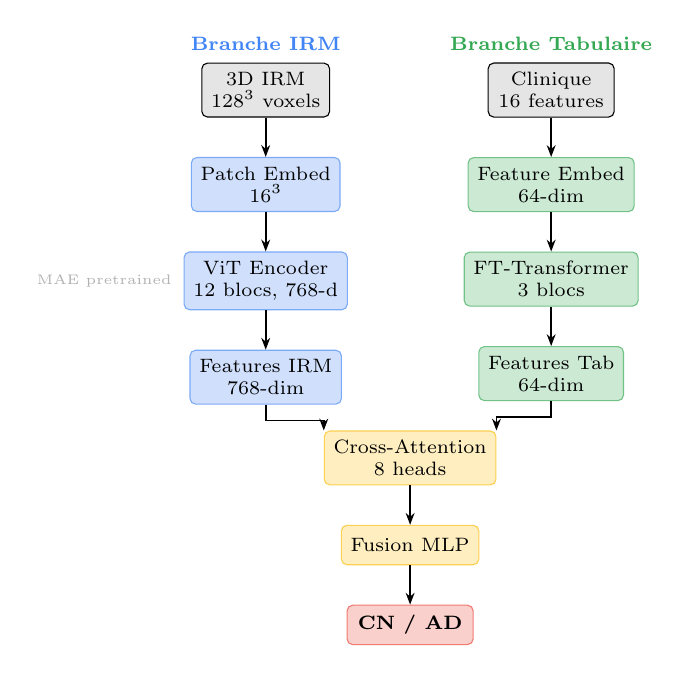
\begin{tikzpicture}[
    node distance=0.5cm and 0.8cm,
    box/.style={rectangle, draw, rounded corners=2pt, minimum width=1.6cm, minimum height=0.5cm, align=center, font=\scriptsize},
    input/.style={box, fill=gray!20},
    mri/.style={box, fill=mricolor!25, draw=mricolor!70},
    tab/.style={box, fill=tabcolor!25, draw=tabcolor!70},
    fusion/.style={box, fill=fusioncolor!25, draw=fusioncolor!70},
    output/.style={box, fill=outputcolor!25, draw=outputcolor!70},
    arrow/.style={-{Stealth[length=1.5mm]}, semithick},
    lbl/.style={font=\tiny, text=gray!60}
]

% MRI Branch
\node[input] (mri_in) {3D IRM\\$128^3$ voxels};
\node[mri, below=of mri_in] (patch) {Patch Embed\\$16^3$};
\node[mri, below=of patch] (vit) {ViT Encoder\\12 blocs, 768-d};
\node[mri, below=of vit] (mri_f) {Features IRM\\768-dim};

% Tabular Branch
\node[input, right=2cm of mri_in] (tab_in) {Clinique\\16 features};
\node[tab, below=of tab_in] (femb) {Feature Embed\\64-dim};
\node[tab, below=of femb] (ftt) {FT-Transformer\\3 blocs};
\node[tab, below=of ftt] (tab_f) {Features Tab\\64-dim};

% Fusion - use coordinate midway
\path (mri_f) -- (tab_f) coordinate[midway] (mid);
\node[fusion, below=0.7cm of mid] (cross) {Cross-Attention\\8 heads};
\node[fusion, below=of cross] (fmlp) {Fusion MLP};

% Output
\node[output, below=of fmlp] (cls) {\textbf{CN / AD}};

% Arrows
\draw[arrow] (mri_in) -- (patch);
\draw[arrow] (patch) -- (vit);
\draw[arrow] (vit) -- (mri_f);
\draw[arrow] (tab_in) -- (femb);
\draw[arrow] (femb) -- (ftt);
\draw[arrow] (ftt) -- (tab_f);
\draw[arrow] (mri_f.south) -- ++(0,-0.2) -| (cross.north west);
\draw[arrow] (tab_f.south) -- ++(0,-0.2) -| (cross.north east);
\draw[arrow] (cross) -- (fmlp);
\draw[arrow] (fmlp) -- (cls);

% Labels
\node[lbl, left=0.03cm of vit] {MAE pretrained};

% Branch titles
\node[above=0.03cm of mri_in, font=\scriptsize\bfseries, text=mricolor] {Branche IRM};
\node[above=0.03cm of tab_in, font=\scriptsize\bfseries, text=tabcolor] {Branche Tabulaire};

\end{tikzpicture}
}%

\vspace{1mm}
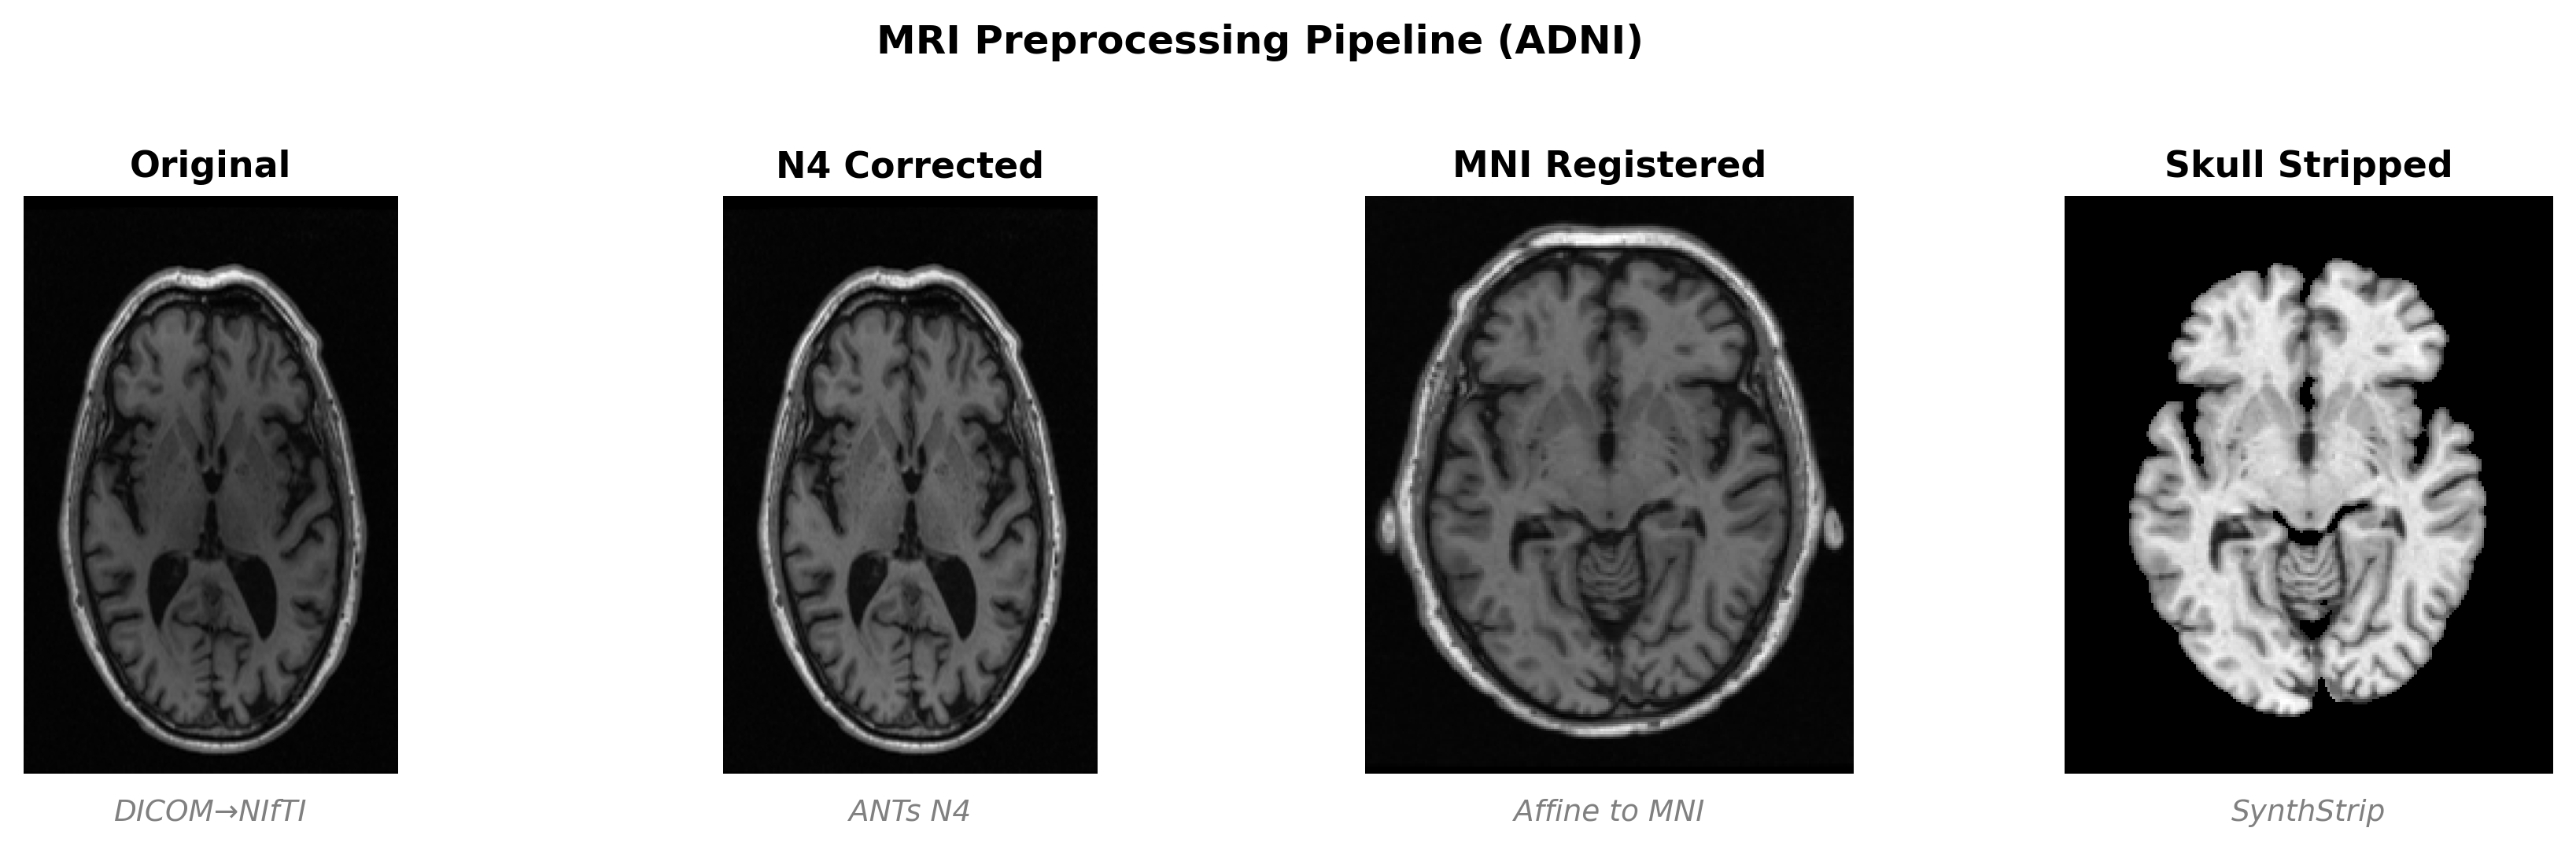
\includegraphics[width=\columnwidth]{../paper/figures/preprocessing_pipeline.png}

\end{column}
\end{columns}

\end{frame}


% ============================================================
% SLIDE 2 : Résultats & Explicabilité
% ============================================================
\begin{frame}{R\'{e}sultats \& Explicabilit\'{e}}

\begin{columns}[T]

% --- Left column: Results tables ---
\begin{column}{0.50\textwidth}

\vspace{-2mm}
\textbf{\color{mricolor} Transformers (ViT + FT-Transformer)}

\vspace{1mm}
\centering
\scriptsize
\begin{tabular}{@{}lcccc@{}}
\toprule
\textbf{Mod\`{e}le} & \textbf{Acc} & \textbf{Sens} & \textbf{Sp\'{e}c} & \textbf{AUC} \\
\midrule
IRM seule (ViT) & 83.3 & 56.2 & 90.8 & .826 \\
Tabulaire (FT-T) & 84.9 & 83.5 & 85.2 & .925 \\
\rowcolor{fusioncolor!20}
\textbf{Fusion ViT+FT-T} & \textbf{92.4} & \textbf{78.8} & \textbf{96.2} & \textbf{.959} \\
\bottomrule
\end{tabular}

\vspace{2.5mm}
\raggedright
\textbf{\color{outputcolor} CNN 3D (ResNet3D) -- single split}

\vspace{1mm}
\centering
\scriptsize
\begin{tabular}{@{}lcccc@{}}
\toprule
\textbf{Mod\`{e}le} & \textbf{Acc} & \textbf{Sens} & \textbf{Sp\'{e}c} & \textbf{AUC} \\
\midrule
ResNet3D seul & 87.3 & 76.3 & 90.3 & .914 \\
\midrule
\multicolumn{5}{@{}l}{\textit{Early fusion :}} \\
R3D + MLP & \textbf{93.5} & \textbf{85.9} & 95.6 & .934 \\
R3D + XGBoost & 90.7 & 79.3 & 93.8 & .944 \\
\midrule
\multicolumn{5}{@{}l}{\textit{Late fusion :}} \\
R3D + MLP (weighted) & 91.4 & 86.4 & 92.8 & \textbf{.955} \\
R3D + XGB (weighted) & 92.5 & 82.8 & 95.2 & .952 \\
\bottomrule
\end{tabular}

\end{column}

% --- Right column: GradCAM ---
\begin{column}{0.48\textwidth}

\vspace{-2mm}
\textbf{\color{outputcolor} Explicabilit\'{e} -- CNN 3D (ResNet3D)}

\vspace{1mm}
{\scriptsize En parall\`{e}le du ViT, un \textbf{ResNet3D + MLP} (early fusion) a \'{e}t\'{e} entra\^{i}n\'{e} pour l'analyse d'explicabilit\'{e}.}

\vspace{1mm}
\centering
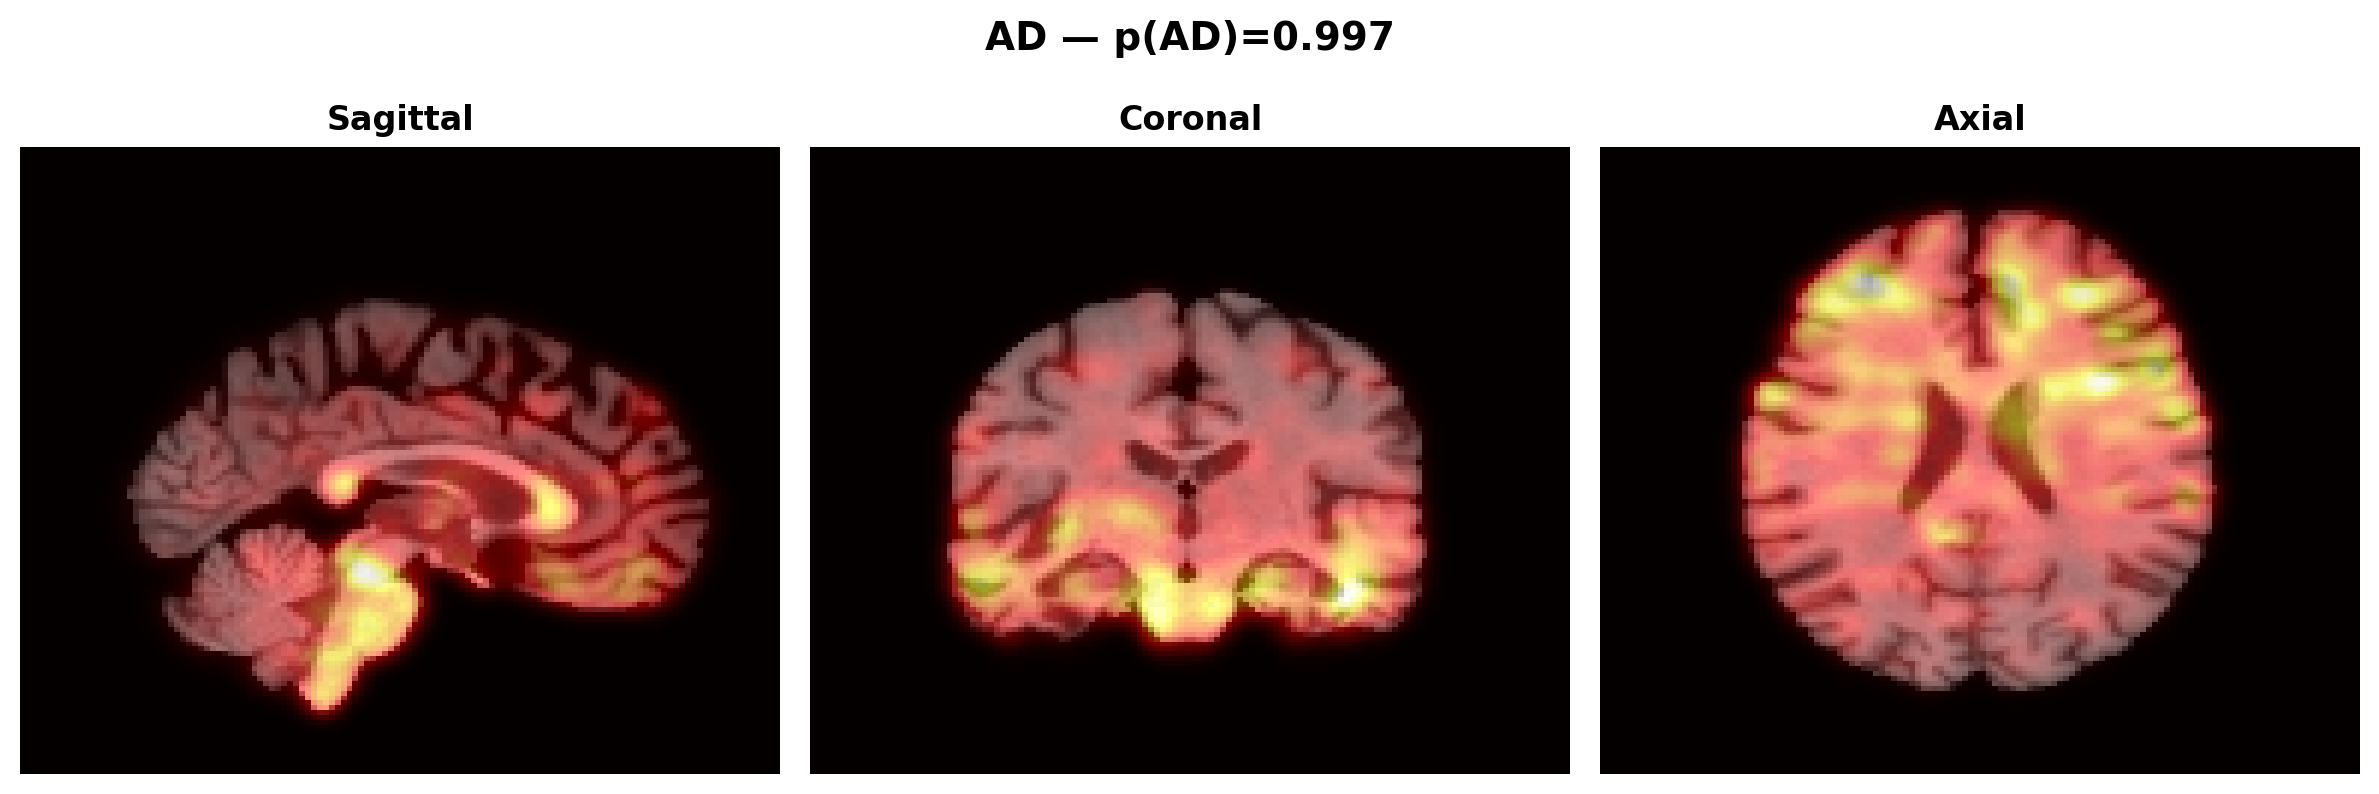
\includegraphics[width=\columnwidth]{../experiments/report_multi_seed/interpretability/mlp_early_fusion/AD_01.png}

\vspace{1mm}
{\scriptsize Integrated Gradients -- Patient AD, p(AD) = 0.997}

\vspace{1mm}
\raggedright
\small
\begin{itemize}\setlength\itemsep{1pt}
    \item Zones activ\'{e}es : \textbf{hippocampe}, \textbf{lobe temporal m\'{e}dial}
    \item R\'{e}gions connues pour l'atrophie AD
    \item Patterns \textbf{coh\'{e}rents} avec la neuropathologie
\end{itemize}

\end{column}
\end{columns}

\end{frame}

\end{document}
